\section{Ontology and knowledge graph design}\label{sec:ontology}

\subsection{T-Box: classes, properties and constructs}
The schema (\texttt{Ontology/qualifypath.ttl}, \statTbox{} triples) defines \statClasses{} classes,
\statObjProps{} object properties and \statDataProps{} datatype properties in the namespace
\texttt{qp:~<http://example.org/qualifypath/ontology\#>}. The match hierarchy separates what has happened from
what is still to come: \texttt{CompletedMatch} (with subclasses \texttt{DecidedMatch} and
\texttt{NoResultMatch}) is disjoint with \texttt{ScheduledMatch}. Tournament rules (\texttt{PointsRule},
\texttt{QualificationRule}, \texttt{TieBreakCriterion}) are \emph{data} attached to a season, so a different
tournament only needs different rule instances. Standings live in \texttt{StandingEntry} resources whose status
subclasses are filled by rules, never loaded (\figref{fig:ontology_schema.jpg}).

\begin{figure}[H]\centering
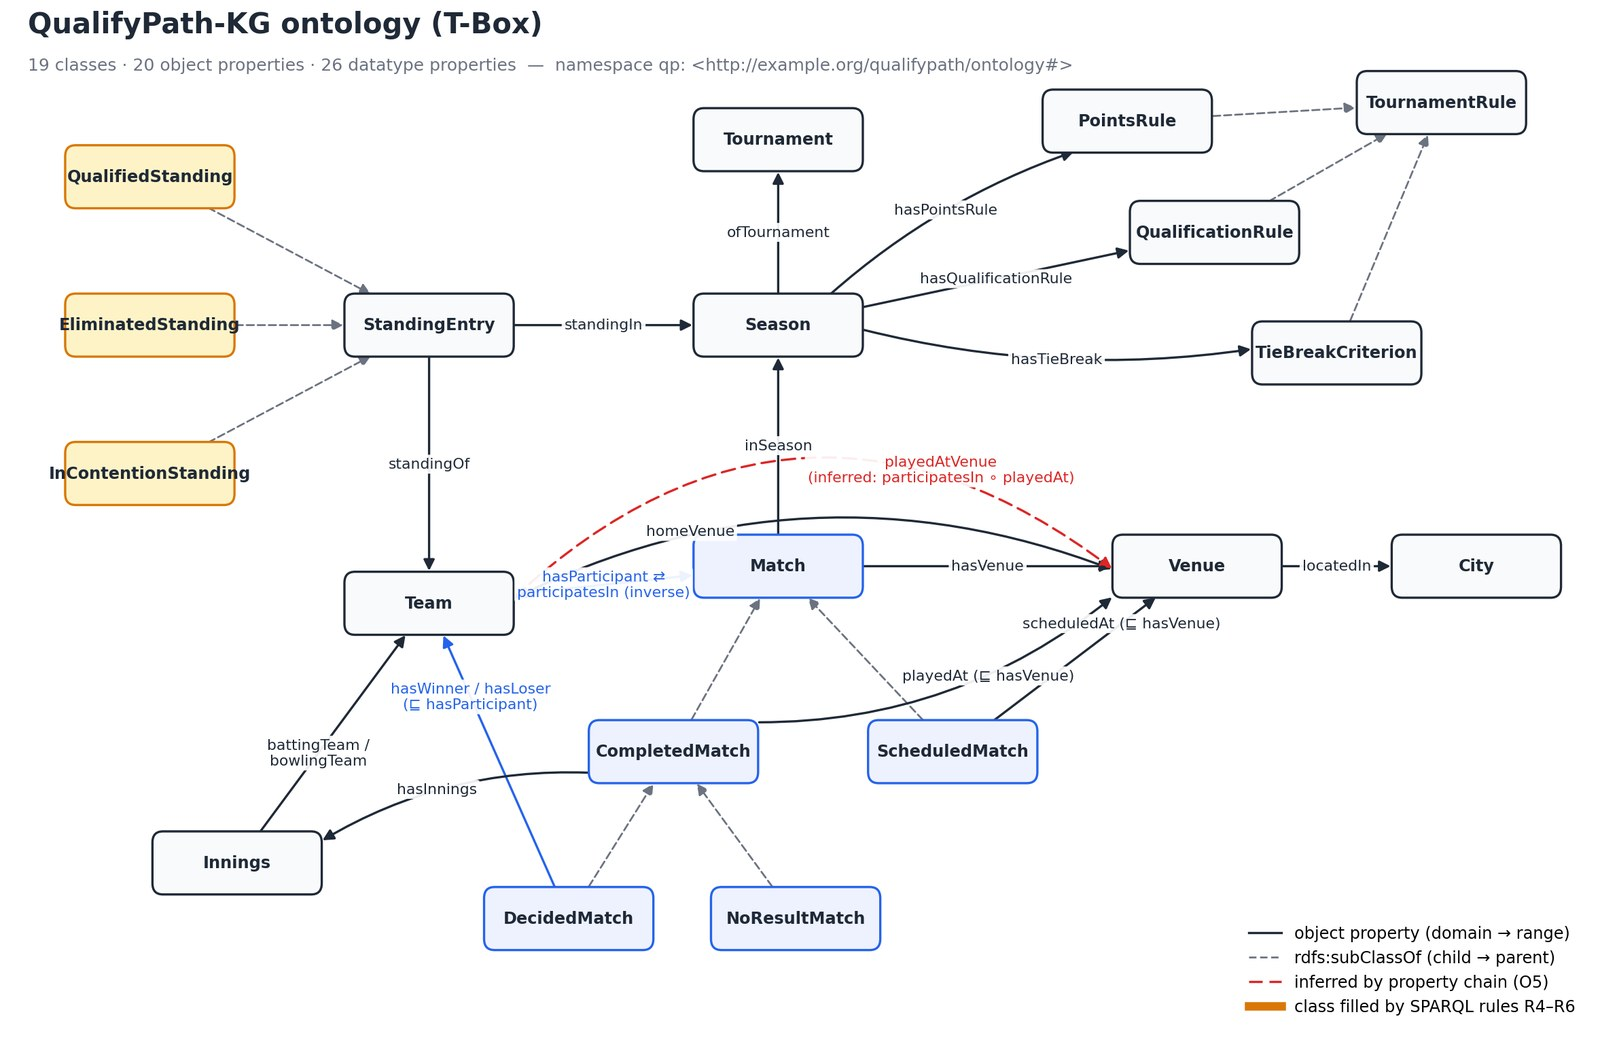
\includegraphics[width=\linewidth]{figures/ontology_schema.jpg}
\caption{Ontology (T-Box): classes, subclass links and object properties (domain $\rightarrow$ range). The red
dashed edge is inferred by a property chain; amber classes are filled by SPARQL rules R4--R6.}
\label{fig:ontology_schema.jpg}
\end{figure}

\begin{table}[H]\centering\small
\begin{tabular}{p{0.7cm}p{6.6cm}p{7.6cm}}
\toprule
\textbf{Code} & \textbf{Construct} & \textbf{What the reasoner infers} \\ \midrule
O1 & \texttt{hasWinner}, \texttt{hasLoser} \texttt{rdfs:subPropertyOf} \texttt{hasParticipant} & the winner and loser of a match are its participants \\
O2 & \texttt{participatesIn} \texttt{owl:inverseOf} \texttt{hasParticipant} & Team $\rightarrow$ participatesIn $\rightarrow$ Match without storing it twice \\
O3 & \texttt{hasWinner} \texttt{rdfs:domain} \texttt{DecidedMatch} & a match with a winner is a DecidedMatch \\
O4 & \texttt{DecidedMatch}, \texttt{NoResultMatch} \texttt{rdfs:subClassOf} \texttt{CompletedMatch} & decided and abandoned matches count as completed \\
O5 & \texttt{playedAtVenue} \texttt{owl:propertyChainAxiom} (\texttt{participatesIn} \texttt{playedAt}) & Team $\rightarrow$ playedAtVenue $\rightarrow$ Venue \\
\bottomrule
\end{tabular}
\caption{Reasoning-enabling constructs. Constraints (consistency checks): CompletedMatch $\sqcap$ ScheduledMatch
$=\emptyset$, a Match has exactly two participants, a DecidedMatch exactly one winner, status classes are
disjoint.}
\end{table}

OWL~2~RL \citep{w3c2012owl2profiles} was chosen because it is the rule-based profile that both
\texttt{owlrl} (Python) and GraphDB's OWL2-RL ruleset implement, and it supports every construct above,
including property chains. Arithmetic (points, NRR, positions) is outside OWL, so it is done by SPARQL Update
rules (Section~\ref{sec:sparql}).

\textbf{Improvements in Iteration 2.} \texttt{playedAt} is now restricted to completed matches and a new
\texttt{scheduledAt} (both sub-properties of \texttt{hasVenue}) covers fixtures, after the reasoner showed that
the venue chain also counted future fixtures; \texttt{oversPerSide} handles rain-shortened matches; and the
tie-break order follows IPL clause 16.10.2.

\subsection{A-Box and URI design}
The instance data (\texttt{RDF\_Knowledge\_Graph/ipl2026\_abox.ttl}) has \statAbox{} triples; with the
ontology the graph holds \statExplicit{} explicit triples --- well above the 500 required --- and grows to
\statFull{} after OWL~2~RL reasoning (\statInferred{} inferred) and the rules (\statRule{} rule-derived).
Decided matches are stored only as \texttt{qp:Match} with \texttt{hasWinner}/\texttt{hasLoser}; that they are
completed, decided and who participated is left to the reasoner.

\begin{table}[H]\centering\small
\begin{tabular}{p{2.3cm}p{6.4cm}p{6.2cm}}
\toprule
\textbf{Resource} & \textbf{Pattern} (\texttt{\ldots/resource/}) & \textbf{Example} \\ \midrule
Ontology term & \texttt{\ldots/ontology\#<Term>} & \texttt{qp:DecidedMatch} \\
Team & \texttt{team/<official abbreviation>} & \texttt{team:RR} \\
Venue / City & \texttt{venue/<slug>}, \texttt{city/<slug>} & \texttt{venue:eden-gardens} \\
Season & \texttt{season/<tournament>-<year>} & \texttt{season:IPL-2026} \\
Match & \texttt{match/<season>-M<number>} & \texttt{match:IPL-2026-M32} \\
Innings & \texttt{innings/<match>-<n>} & \texttt{innings:IPL-2026-M32-1} \\
Rule & \texttt{rule/<season>-<rule>} & \texttt{rule:IPL-2026-tiebreak-1} \\
Standing & \texttt{standing/<season>-<team>} (rule-created) & \texttt{standing:IPL-2026-RR} \\
\bottomrule
\end{tabular}
\caption{URI design: readable, stable identifiers from official codes; season-scoped where a resource belongs to
one season; names kept in \texttt{rdfs:label} so spelling variants never create duplicates.}
\end{table}

\subsection{Knowledge graph visualisation}
\begin{figure}[H]\centering
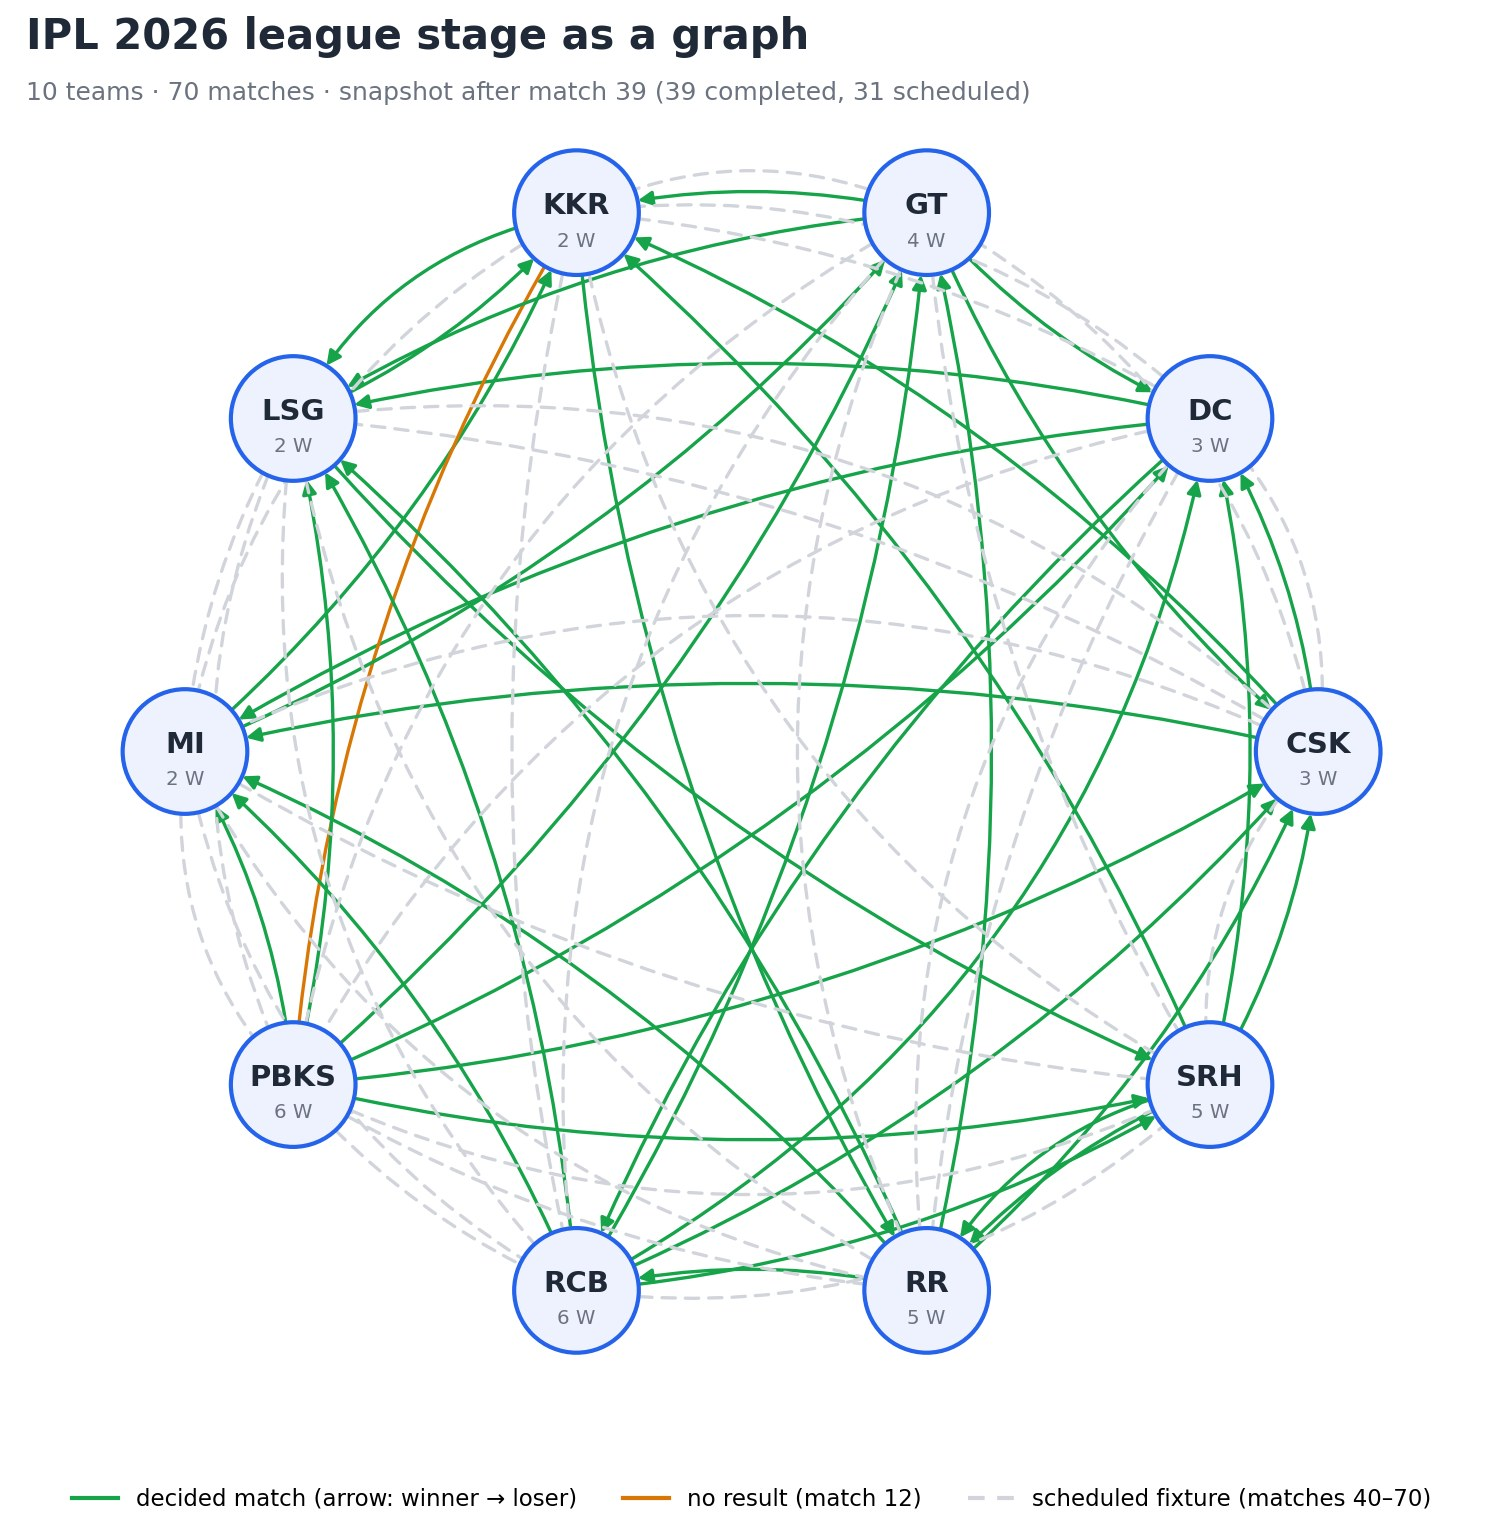
\includegraphics[width=0.78\linewidth]{figures/season_graph.jpg}
\caption{The league stage as a graph: ten teams, each of the 70 matches an edge (winner $\rightarrow$ loser,
no result, or scheduled).}
\end{figure}
\shot[0.92\linewidth]{rr_neighbourhood.jpg}{Instance level: RR, its 14 matches, opponents and venue cities.}
\shot[0.9\linewidth]{graphdb_class_hierarchy.jpg}{GraphDB class hierarchy of the loaded repository
(\texttt{qualifypath-ipl2026}, OWL2-RL ruleset).}
\shot[0.9\linewidth]{graphdb_visual_graph_match03.jpg}{GraphDB visual graph of match~3: the types
\emph{Completed match} and \emph{Decided match} are inferred, not stored.}
\shot[0.9\linewidth]{graphdb_visual_graph_RR.jpg}{GraphDB visual graph of RR: its matches, the venues it has
played at (inferred) and its standing entry.}
